%%=============================================================================
%% Proof of concept
%%=============================================================================
\usepackage{graphicx}
\graphicspath{ {./graphics/} }
\chapter{\IfLanguageName{dutch}{Proof Of Concept}{Proof Of Concept}}%

In dit hoofdstuk wordt de proof of concept uitgewerkt. De recent verkregen informatie wordt hierbij omgezet in de praktijk. De Proof Of Concept zal een beeld vormen van de oplossing voor het gestelde probleem. Als eerst zal er gekeken worden naar de gebruikte netwerkopstelling binnen Azure.
Vervolgens zal de gebruikte infrastructuur aan bod komen. Daarnaast zal er dieper worden ingegaan op Ansible en de bijhorende playbooks die zorgen voor de configuratie van de firewall. Verder wordt er gekeken naar de uitwerking van het powershell script dan instaat voor het uitvoeren van controles op de ingevoerde data door de klant. Dit script zal alle zaken die hiervoor werden besproken samenbrengen tot 1 werkende geheel. 

\newpage

\section{Netwerkopstelling}
De netwerkopstelling die gebruikt wordt voor de Proof of Concept bestaat uit 2 virtuele machines elk in hun eigen subnet respectievelijk. In het eerste subnet met netwerkadres 172.22.2.0 bevindt zich een webserver met het adres 172.22.2.5. In het tweede subnet met netwerkadres 172.22.1.0 bevindt zich een host met het adres 172.22.1.5. Tussen deze twee subnets bevindt zich een firewall in de vorm van een Network Virtual Appliance (NVA) van fortinet. Deze netwerkopstelling zorgt voor een ideale testomgeving. De mogelijkheid voorzien dat de host de webserver kan bereiken aan de hand van geautomatiseerde firewallrules waarop controle is uitgevoerd, is het uitendelijke doel van deze Proof of Concept. 
\subsection{Topologie}
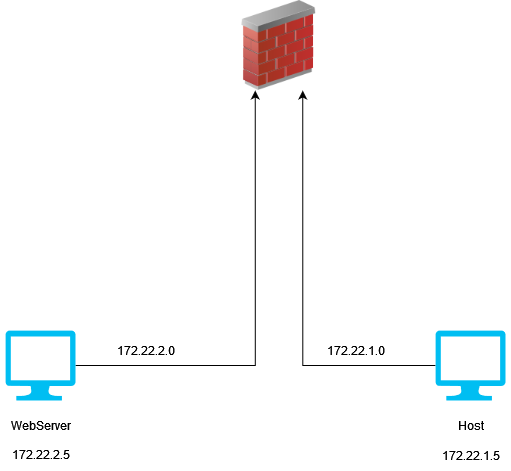
\includegraphics[width=100mm]{bachproef/graphics/topologie.png}
%%=============================================================================
%% Methodologie
%%=============================================================================

\chapter{\IfLanguageName{dutch}{Methodologie}{Methodology}}%
\label{ch:methodologie}
Dit onderzoek zal in verschillende delen verlopen. In hoofdstuk twee werd er vooral informatie vergaard om het probleem zo goed mogelijk te begrijpen. Deze informatie werd verkregen aan de hand van een relevante literatuurstudie. Ook zal er beroep gedaan worden op interviews met belanghebbenden om op deze manier een requirements-analyse te kunnen uitvoeren. Dit zal ervoor zorgen dat er een optimale oplossing komt voor het beschreven probleem. De informatie wordt vervolgens gebruikt voor het opmaken van een Proof-of-Concept, waarin alle informatie zal toegepast worden in de praktijk. Dit Proof-of-Concept zal uiteindelijk ook het eindproduct zijn, waarin de oplossing van het probleem wordt weergegeven. Hierover zal ook een presentatie gegeven worden. Voor dit onderdeel wordt er beroep gedaan op communicatie met de copromoter en het bedrijf waarvoor dit onderzoek wordt uitgevoerd. Hiervoor zal een uitgebreide verzameling van software en hardware nodig zijn. Zo zal het mogelijk moeten zijn om gebruik te maken van alle Microsoft Azure features voor een zo'n specifiek mogelijke oplossing. Op deze manier kan er een realistisch scenario worden opgebouwd. Verder zal er ook eventueel beroep gedaan worden op een webapplicatie waarmee het mogelijk is firewall regels in te geven. Dit zal een zeer simpele applicatie zijn, geschreven in JavaScript. Deze applicatie is essentieel voor het oplossen van het gegeven probleem. Het is de bedoeling dat een klant aan de hand van een webapplicatie firewall regels kan doorsturen naar een firewall. Deze regels zullen worden opgenomen in een JSON-file. Op deze manier kan deze makkelijk worden geïmplementeerd in een script. Deze scripts worden gemaakt met Ansible in combinatie met een andere tool.  
Het zou kunnen dat tijdens het uitvoeren van het effectief onderzoek een betere oplossing wordt gevonden.
Concreet wordt er een Azure netwerk opgezet met een Network Virtual Appliance van het merk Fortigate. Op dit netwerk zal dan ook een webapplicatie draaien. Vervolgens worden er templates gebouwd, in verschillende Infrastructure as Code tools, voor het deployen van de gewenste firewall regels. Vervolgens zal er ook gekeken worden of deze manier van werken ook toegepast kan worden op een firewall van een andere vendor zoals Cisco. Voor dit onderdeel wordt ongeveer 40 uur geschat. Ten slotte worden de resultaten geanalyseerd en samen gebundeld in een concrete conclusie. 
%% TODO: Hoe ben je te werk gegaan? Verdeel je onderzoek in grote fasen, en
%% licht in elke fase toe welke stappen je gevolgd hebt. Verantwoord waarom je
%% op deze manier te werk gegaan bent. Je moet kunnen aantonen dat je de best
%% mogelijke manier toegepast hebt om een antwoord te vinden op de
%% onderzoeksvraag.



